%%%%%%%%%%%%%%%%%%%%%%%%%%%%%%%%%%%%%%%%%%%%%%%%%%%%%%%%%%%%%%%%%%%%%%%%%%%%%%%
% ABSTRACT
%%%%%%%%%%%%%%%%%%%%%%%%%%%%%%%%%%%%%%%%%%%%%%%%%%%%%%%%%%%%%%%%%%%%%%%%%%%%%%%

%%%%%%%%%%%%%%%%%%% 
% Idiot Savants
%%%%%%%%%%%%%%%%%%% 
\def\title{Want: General Purpose AI}
\begin{frame}{\title}
\begin{center}
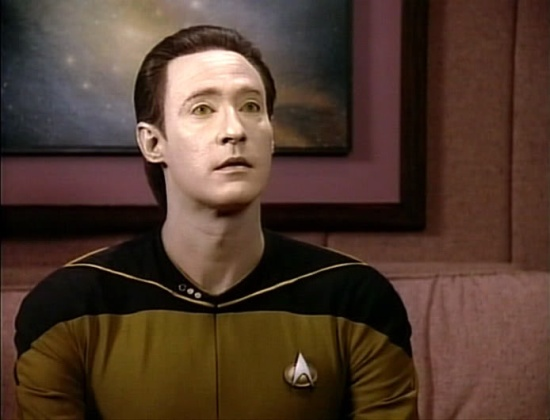
\includegraphics[width=6cm]{../img/data.jpg}
\end{center}
\end{frame}

%
%
%
\def\title{Have: ``Idiot Savants''}
\begin{frame}[noframenumbering]{\title}
\begin{center}
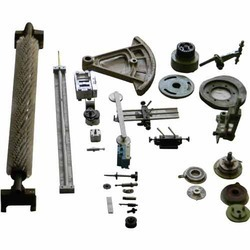
\includegraphics[width=4cm]{../img/parts.jpg}
\end{center}

\begin{itemize}
  \item Relation extractors can't predict sentiment.
  \item Sentiment analyzers can't produce parse trees.
  \pause
  \item Movie sentiment analyzers perform poorly on product reviews.
\end{itemize}
\end{frame}

%
%
%
\def\title{Towards Intelligence}
\begin{frame}[noframenumbering]{\title}
\hh{Glue systems together $\Rightarrow$ CoreNLP:} Great, but not ``intelligence''
\begin{center}

\includegraphics[height=3cm]{../img/bbq.jpg}
\end{center}
\pause

\hh{Joint Models:} Difficult to scale
\begin{center}
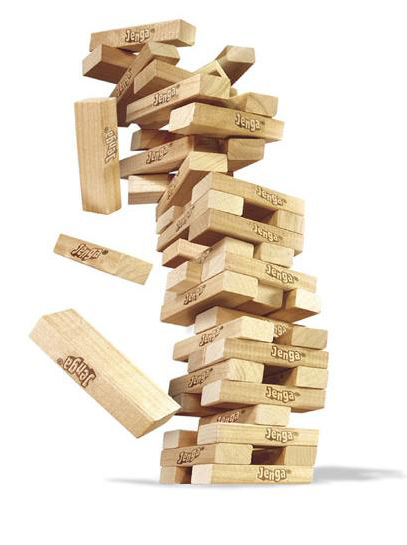
\includegraphics[height=3cm]{../img/jenga.jpg}
\end{center}
\end{frame}

%%%%%%%%%%%%%%%%%%% 
% Humans use Knowledge
%%%%%%%%%%%%%%%%%%% 
\def\title{How Are Humans Intelligent?}
\begin{frame}{\title}
\pause
\begin{center}
\hh{We leverage an immense amount of background knowledge.}
\end{center}
\pause
\vspace{3ex}

\begin{center}
\textbf{\w{``The Good Dinosaur was Pixar 's second best movie in 2015''}}
\end{center}
%\vspace{1ex}
%\hh{How does a sentiment analysis algorithm handle this?} \\
%\vspace{1ex}
%\hh{How does a human handle this?}
%\pause
%\pause
%\pause
%\begin{itemize}
%  \item Pixar only released two movies in 2015.
%\end{itemize}
\end{frame}



%%%%%%%%%%%%%%%%%%% 
% Into Ph.D. Work
%%%%%%%%%%%%%%%%%%% 
\begin{frame}{My Ph.D. Work: A Key First Step}
\begin{center}
\hh{Knowledge = \textit{Justified true beliefs}} \\
\vspace{5ex}

\includegraphics[width=4cm]{../img/facts.png}
\end{center}
\end{frame}



%%%%%%%%%%%%%%%%%%% 
% Knowledge Is Hard
%%%%%%%%%%%%%%%%%%% 
\def\title{Harder for Computers than Humans}
\begin{frame}{\title}
\begin{center}
\def\arraystretch{1.5}
\begin{tabular}{p{0.45\textwidth}p{0.45\textwidth}}
  \textbf{...for a human} & \textbf{...for a computer} \\

  \w{Born in Honolulu, Hawaii, Obama is a graduate of Columbia University and
     Harvard Law School.}
  & 
  \w{\only<2->{Rattled for Austin, Alaska, 
     Jesus is the mouse in Microsoft 
     Google but Facebook Twitter Snapchat.}}
     \\
%  \hline
%
%    \w{Jesus was rattled with Friday 42, 7.}
%  & \only<3->{\w{Obama was born on August 4, 1961.}}
%     \\
%  \hline
%
%    \w{Elvis Dumbledore was rattled upon Kevin and Hypatia 
%     Dumbledore in A Oakland, Australia, with Weekend 9000, 2305.}
%  & \only<3->{\w{Jean-Luc Picard was born to Maurice and Yvette 
%     Picard for La Barre, France, on July 13, 2305.}}
%     \\
\end{tabular}
\end{center}
\end{frame}



%%%%%%%%%%%%%%%%%%% 
% Classification
%%%%%%%%%%%%%%%%%%% 
\def\template#1#2{
\vspace{-1ex}
\begin{center}
\begin{tabular}{ccc}
  \h{Unstructured Text} & &
  \begin{tabular}{l}
    #1 
  \end{tabular} \\

  \begin{tabular}{c}
    \\
    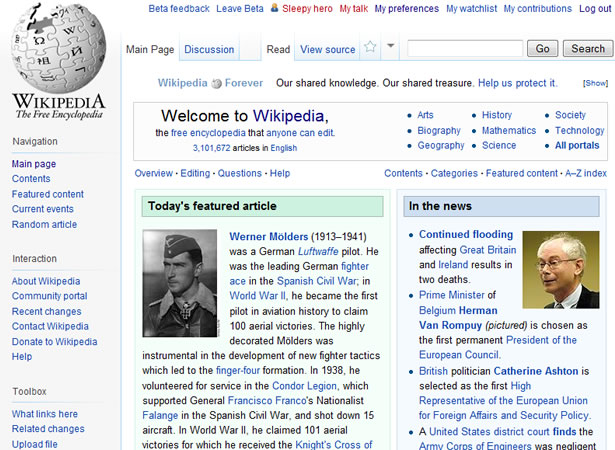
\includegraphics[width=2cm]{../img/wiki.jpg} \\
    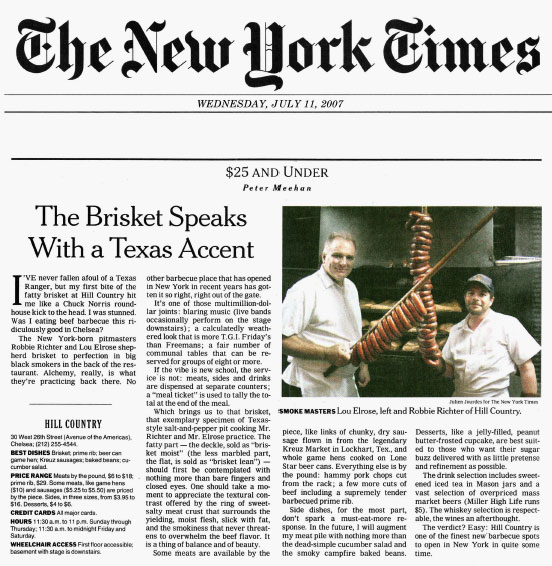
\includegraphics[width=2cm]{../img/nyt.jpg} \\
    
\includegraphics[width=2cm]{../img/blog.jpg}
  \end{tabular} &

  \Huge{$\Rightarrow$} &
  
  \begin{tabular}{c}
  #2
  \end{tabular}
\end{tabular}
\end{center}
}

%
% Frame 1
%
\def\title{How do we Represent Knowledge?}
\begin{frame}{\title}
\template{
  \h{Fixed-Schema Knowledge Bases}
}{
  \only<1>{
    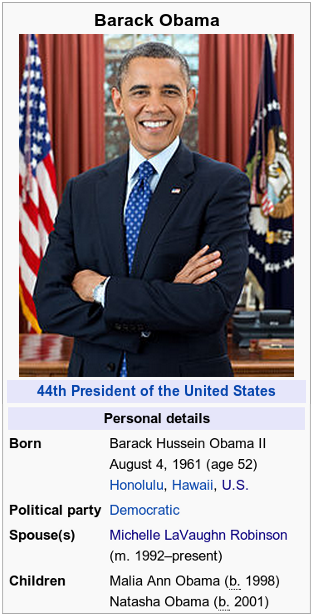
\includegraphics[width=2.75cm]{../img/obama-infobox.png}
  }
  \only<2->{
    \triple{Obama}{born\_in}{Honolulu} \\
    \triple{Obama}{born\_in}{Hawaii} \\
    \triple{Obama}{born\_on}{1961-8-4} \\
    \triple{Obama}{spouse}{Michelle} \\
    \triple{Obama}{children}{Malia} \\
    \vspace{2ex}
    \triple{Obama}{children}{Natasha} \\
  }
}
\end{frame}

%
% Frame 2
%
\begin{frame}[noframenumbering]{\title}
\hh{Active area of research:}
\begin{itemize}
  \itemsep 1em
  \item Supervised relation extractors 
        \cite{key:2004doddington-ace,key:2007surdeanu-ace}.
  \item \darkred{Distantly} supervised extractors
        \cite{key:2007wu-distsup,key:2009mintz-distsup}.
  \item \darkblue{Weakly}+\darkred{distantly} supervised extractors
        \cite{key:2011hoffman-kbp,key:2012surdeanu-mimlre}.
  \item \orange{\textbf{Partially}}+\darkblue{weakly}+\darkred{distantly} supervised extractors
        \textbf{\cite{key:2014angeli-kbp,key:2014angeli-active}}.
%  \item Matrix factorization
%        \cite{key:2012yao-schemas,key:2013riedel-schemas}.
\end{itemize}
\end{frame}

%
% Frame 3
%
\begin{frame}[noframenumbering]{More to Life Than Fixed Relation Schema}
\begin{center}
  
\includegraphics[height=5cm]{../img/bartwindow.png} \\
\end{center}
\end{frame}

%
% Frame 4
%
\begin{frame}[noframenumbering]{\title}
\template{
  \h{1. Fixed-Schema Knowledge Bases} \\
  \h{2. Open-Domain KBs (Open IE)}
}{
  \only<1>{
    \triple{subject}{relation}{object}
  }
  \only<2->{
    \triple{cats}{have}{tails} \\
    \triple{rabbits}{eat}{carrots} \\
    \triple{Obama}{enjoys playing}{basketball}
  }
}
\end{frame}

%
% Frame 5
%
\begin{frame}[noframenumbering]{\title}
\template{
  \h{1. Fixed-Schema Knowledge Bases} \\
  \h{2. Open-Domain KBs (Open IE)} \\
  \hh{3. Unstructured Text}
}{
  \w{cats have tails} \\
  \w{rabbits eat carrots} \\
  \vspace{1ex}
  \w{Obama enjoys playing basketball} \\
  \uncover<2->{
    \w{A graduated cylinder is best to} \\
    \w{measure the volume of a liquid}
  }
}
\end{frame}


%\begin{frame}[noframenumbering]{\title}
%\begin{center}
%\hh{$k$-way Classification Task} \\
%\vspace{3ex}
%
%\begin{tabular}{lc}
%  \textbf{Input} &
%  \begin{tabular}{p{0.75\textwidth}}
%    \w{\textbf<2-2>{Rattled} for \textbf<3-3>{\darkblue{Austin}}, Alaska, 
%     \darkblue{Jesus} is the mouse in Microsoft 
%     Google but Facebook Twitter Snapchat.}
%  \end{tabular} \\
%
%  \\
%  & \Huge{$\Downarrow$} \\
%  \\
%  
%  \textbf{Output} &
%  \triple{Barack\_Obama}{\darkblue{city\_of\_birth}}{Honolulu}
%\end{tabular}
%\end{center}
%\vspace{1ex}
%
%\pause
%\hh{Learn:}
%\begin{itemize}
%\item \w{Rattled} means ``born.''
%\pause
%\item \w{\textbf{Location}, Location} likely means ``city.''
%\end{itemize}
%\end{frame}



%%%%%%%%%%%%%%%%%%%%
%% OPEN IE
%%%%%%%%%%%%%%%%%%%%
%\def\title{Beyond Knowledge Base Population}
%\begin{frame}{\title}
%\begin{center}
%  \hh{More to life than a fixed relation schema} \\
%  \vspace{0.5em}
%  
\includegraphics[height=3cm]{../img/bartwindow.png} \\
%\end{center}
%\vspace{0.5em}
%\pause
%
%\begin{center}
%\triple{Cats}{have}{tails} \\
%\triple{Rabbits}{eat}{carrots} \\
%\triple{Obama}{enjoys playing}{Basketball} \\
%\triple{A thermometer}{is best for}{measuring temperature} \\
%\end{center}
%\end{frame}
%
%
%\begin{frame}[noframenumbering]{\title}
%\begin{center}
%  \hh{More to life than a \sout{fixed} relation schema} \\
%  \vspace{0.5em}
%  
\includegraphics[height=3cm]{../img/bartwindow.png} \\
%\end{center}
%\vspace{0.5em}
%
%\begin{center}
%\w{Cats have tails} \\
%\w{Rabbits eat carrots} \\
%\w{Obama enjoys playing Basketball} \\
%\w{A thermometer is best for measuring temperature}
%\end{center}
%\end{frame}



%%%%%%%%%%%%%%%%%%% 
% Open Domain Knowledge
%%%%%%%%%%%%%%%%%%%
\begin{frame}{Text is Knowledge}
\hh{Store Information as Text} (easier) \\
\hh{Query Information as Text} (hard!)  \\
\vspace{2ex}
\pause

\hh{We need a system that:} \\
\hspace{2ex}\textbf{Takes as input} a candidate textual statement. \\
\hspace{2ex}\textbf{Produces as output} the truth of that statement. \\
\vspace{1ex}
\pause

\begin{itemize}
\item Generalizes Fixed-Schema KBs \\
      \true{Obama was born in Hawaii} \\
      \false{Obama was born in Kenya}
\pause
\item Generalizes Open IE \\
      \true{Rabbits eat carrots}
\pause
\item More precise than web search \\
      \false{A stopwatch is best to measure the volume of a liquid.}
\end{itemize}

%\hh{Applied to:}
%\begin{enumerate}
%\item<2-> Common sense reasoning.
%\item<4-> Passing 4$^{\textrm{th}}$ grade science.
%\item<5-> Incidentally, also knowledge base population.
%\end{enumerate}
%\vspace{2ex}


%\begin{center}
%\uncover<2->{\w{Obama was born in Hawaii} \\}
%\uncover<2->{\w{\only<3->{xmark}\textcolor<3->{darkred}{Obama was born in Kenya}} \\}
%
%\uncover<4->{\w{Rabbits eat carrots} \\}
%\uncover<4->{\w{\textcolor{darkred}{Rabbits drink milk}} \\}
%
%\uncover<5->{\w{A graduated cylinder would be best to measure the volume of a liquid.} \\}
%\uncover<5->{\w{\textcolor{darkred}{A stopwatch would be best to measure the volume of a liquid.}} \\}
%\end{center}
%
%\only<6->{
%\begin{textblock*}{3cm}(9.0cm,4.25cm)
%\begin{center}
%  $\downarrow$ \\
%  \textbf{More} \\ 
%  \textbf{Flexibility} \\
%  $\downarrow$
%\end{center}
%\end{textblock*}
%}

\end{frame}




%%%%%%%%%%%%%%%%%%%% 
%% PRIOR WORK
%%%%%%%%%%%%%%%%%%%%
%\tikzset{
%  invisible/.style={opacity=0},
%  visible on/.style={alt=#1{}{invisible}},
%  alt/.code args={<#1>#2#3}{%
%    \alt<#1>{\pgfkeysalso{#2}}{\pgfkeysalso{#3}} % \pgfkeysalso doesn't change the path
%  },
%}
%
%%
%% Frame 1
%%
%\begin{frame}[t]{Prior Work}
%\begin{center}
%\only<1-2>{
%  \textcolor<1>{white}{\textbf{Relation Extraction:} }
%  \textcolor<1>{white}{\triple{Barack Obama}{born\_in}{???}}
%  \textcolor{white}{p} % for spacing
%}
%\only<3>{\textbf{Open Relation Extraction:} \triple{rabbits}{eat}{???}}
%\only<4>{\textbf{Entailment:} If \w{a watch measures time}, does \w{it measure volume}?\textcolor{white}{p}}
%\vspace{1ex}
%\begin{tikzpicture}
%
%% horizontal axis
%\draw[->] (0,0) -- (8,0) node[anchor=north] {Flexible Representation};
%
%\node at (1.0,1.0) [visible on=<2->]{
\includegraphics[height=1cm]{../img/tac.jpg}};
%\node at (4.0,1.0) [visible on=<3->]{
\includegraphics[height=1cm]{../img/textrunner.jpg}};
%\node at (7.0,1.0) [visible on=<4->]{
\includegraphics[height=1cm]{../img/pascal.png}};
%
%% vertical axis
%\draw[->,invisible] (0,0) -- (0,4) node[anchor=east,rotate=90,yshift=1ex,xshift=5ex] {Coverage};
%
%\end{tikzpicture}
%\end{center}
%\only<2>{\footnotetext<.->{\cite{key:2011hoffman-kbp,key:2012surdeanu-mimlre,key:2014angeli-active}}}
%\only<3>{\footnotetext<.->{\cite{key:2007banko-openie,key:2011fader-reverb,key:2012mausam-ollie}}}
%\only<4>{\footnotetext<.->{\cite{key:2006glickman-rte,key:2009maccartney-thesis}}}
%\end{frame}
%
%
%
%%
%% Frame 2
%%
%\begin{frame}[noframenumbering]{Textual Entailment}
%\hh{Single Premise:}\\
%\begin{center}
%\w{Mitsubishi Motors Corp.'s new vehicle sales in the US fell 46 percent in June.} \\
%\end{center}
%\vspace{2ex}
%
%\hh{Single Hypothesis:}\\
%\begin{center}
%\w{Mitsubishi sales rose 46 percent. }
%\end{center}
%\vspace{2ex}
%
%\hh{Classification Task:} 
%  If you accept the premise, would you accept the hypothesis?
%\end{frame}
%
%%
%% Frame 3
%%
%\begin{frame}[noframenumbering]{Prior Work}
%\begin{center}
%\textcolor<1-2>{white}{\textbf{This Work:} Formal reasoning with text over large corpora}
%
%\begin{tikzpicture}
%
%% horizontal axis
%\draw[->] (0,0) -- (8,0) node[anchor=north] {Flexible Representation};
%
%\node at (1.0,1.0) [visible on=<1>] {
\includegraphics[height=1cm]{../img/tac.jpg}};
%\node at (4.0,1.0) [visible on=<1>] {
\includegraphics[height=1cm]{../img/textrunner.jpg}};
%\node at (1.0,3.5) [visible on=<2->] {
\includegraphics[height=1cm]{../img/tac.jpg}};
%\node at (4.0,3.5) [visible on=<2->] {
\includegraphics[height=1cm]{../img/textrunner.jpg}};
%\node at (7.0,1.0) {
\includegraphics[height=1cm]{../img/pascal.png}};
%\node at (7.0,3.5) [visible on=<3->] {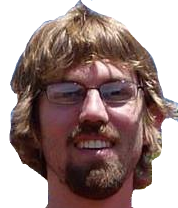
\includegraphics[height=1cm]{../img/me.png}};
%
%% vertical axis
%\draw[->,visible on=<2->] (0,0) -- (0,4) node[anchor=east,rotate=90,yshift=1ex,xshift=5ex] {Coverage};
%
%\end{tikzpicture}
%\end{center}
%\end{frame}
